\section{カッシーニとは}

カッシーニとは,NASA
\footnote{アメリカ航空宇宙局}
とESA
\footnote{欧州宇宙機関}
が開発した土星探査機のこと.1997年にタイタンIVロケット
\footnote{アメリカ空軍がスペースシャトル・チャレンジャー事故後に大型衛星打ち上げ用に開発したロケット.1989年から2005年まで使用された.}
で打ち上げられた.名称は天文学者ジョバンニ・カッシーニに由来する.

\section{カッシーニのミッション}
 カッシーニの主なミッションは,土星の大気や、謎に包まれていた輪の構造、衛星の探査である.特に,衛星タイタンについてはESAが開発した小型探査機ホイヘンスを降下させ,その大気や地形の詳細な探査を行った.
現在,最終ミッションである「グランドフィナーレ」を実行中だ.

\section{土星観測の歴史}
カッシーニの探査対象である土星の大きな特徴は,その大きな輪だ.小型の望遠鏡でも簡単に観測することが出来るので、各地の天文台の観望会などでも人気の天体となっている.

\begin{figure}[htbp]
	\begin{minipage}[t]{0.45\hsize}
        \centering
        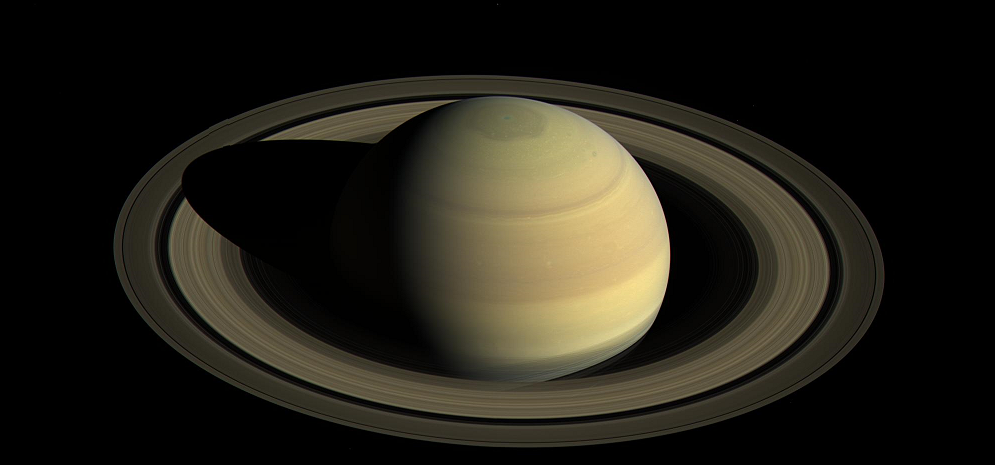
\includegraphics[width=5cm]{img/saturn.png}
        \subcaption{大きな輪が特徴的な土星}
    \end{minipage}
	\begin{minipage}[t]{0.45\hsize}
        \centering
    	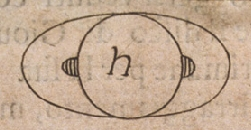
\includegraphics[width=5cm]{img/galileo-saturn-sketch.png}
    	\subcaption{ガリレオによる土星のスケッチ}
    \end{minipage}
\end{figure}

この特徴的な輪を初めて観測したのはガリレオ・ガリレイで,初めて望遠鏡を空に向けた翌年,1610年のことだった.しかし,望遠鏡の精度が低かったため,輪とは判別できず,「耳のようなものがある」と表現した.
また,1612年には輪が地球の正面を向いて輪が見えなくなった
\footnote{土星は回転軸を傾けたまま太陽の周りを公転しているため,地球から見たときに,環がはっきりと見える時期と環がほとんど見えなくなる時期がある.}
ため,ガリレオは困惑し,土星の英語名saturnの由来であるサートゥルヌスの神話のエピソード
\footnote{サートゥルヌスはローマ神話の農耕神で,ギリシャ神話のクロノスと同一視される.シンボルは鎌.
サートゥルヌスには,「自分の子供に殺される」という予言を恐れて,5人の次々に飲み込んでいったという伝承がある.}
になぞらえ,「土星は子供達を飲み込んだのか?」と言ったという.
\footnote{翌年にはまた土星の環が見えるようになったため,ガリレオはさらに困惑した.}

\begin{figure}[h]
\centering
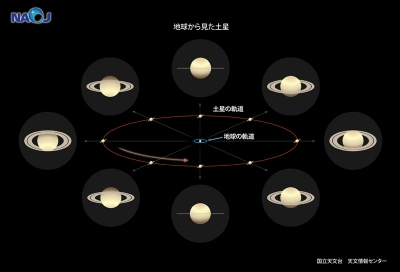
\includegraphics[width=5cm]{img/saturn-ring-dissapear.jpg}
\caption{土星の環の消失現象の仕組み}
\end{figure}

その後,1655年にオランダの天文学者ホイヘンスがこの「耳のようなもの」がディスク状のものであると発表.
さらにホイヘンスは土星本体と輪の間に隙間を発見した.
\footnote{この功績から,土星の輪の隙間の一つは「ホイヘンスの空隙」(間隙,という場合もある)
」という名前がつけられている.}


さらにその後,1787年にはピエール=シモン・ラプラスが土星の環が小さな環の集まりであると提唱,1859年にはジェームズ・クラーク・マクスウェル
\footnote{「マクスウェル方程式」の"あの"マクスウェルである.}
が,土星の環が小天体の集まりで出来ていると提唱した.


その後,土星探査が大きく進展したのは,1979年9月にパイオニア11号
\footnote{NASAの惑星探査計画,パイオニア計画の一環で,パイオニア10号の姉妹機.初の土星探査機である.}
が土星に最接近したときのことだった.
パイオニア10号は土星に21000kmの距離まで接近し,E,F,G環を発見したほか,衛星タイタンの気温が250K程度と測定.
1980年11月にはボイジャー1号が土星に到着,パイオニア11号では得られなかった高画質の画像を得られた.また,ジャー1号はタイタンに接近,タイタンの分厚い大気
\footnote{分厚い大気の層をもつ衛星はタイタンのみである.}
を発見した.
翌年1981年8月には,ボイジャー2号が土星に到着.新たな衛星や空隙を発見した.


パイオニアやボイジャーにより,それまでよく分かっていなかった土星の姿が少しづつ分かってきたが,これらの探査機はあくまで一時的に土星に「立ち寄った」だけで,継続的な土星の探査というのは行っていなかった.


人類が継続的に土星を探査する機会を得るには,今回取り上げるカッシーニが土星に到着する2004年まで待たねばならない.

\section{探査機カッシーニによる土星探査}


探査機カッシーニは,1997年に打ち上げられた後,金星で2回,地球と木星で1回ずつスイングバイを繰り返して,2004年に土星軌道に到達した.
翌年2005年には小型探査機ホイヘンスを衛星タイタンに降下させて詳細な探査を行った他,土星の輪や大気の詳細な構造,衛星の探査を行った.
もともと探査は4年間の予定であったが,探査機の状態が良く,また,タイタンを利用したクローズドスイングバイにより燃料が節約できていたため,探査計画は延長された.
そして,土星軌道投入10周年の2014年に最終ミッション,「グランドフィナーレ」が発表された.

\begin{figure}[htbp]
\centering
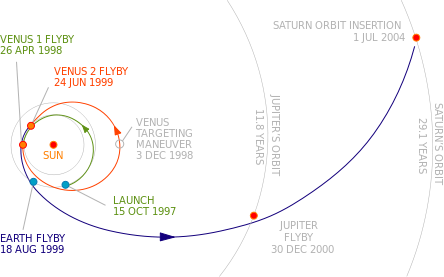
\includegraphics[width=5cm]{img/cassini-orbit.png}
\caption{カッシーニの土星到達までの道のり}
\end{figure}


10年以上にわたるカッシーニの探査は,土星やその輪,衛星に関する様々な成果を生んだ.

\begin{figure}
\centering
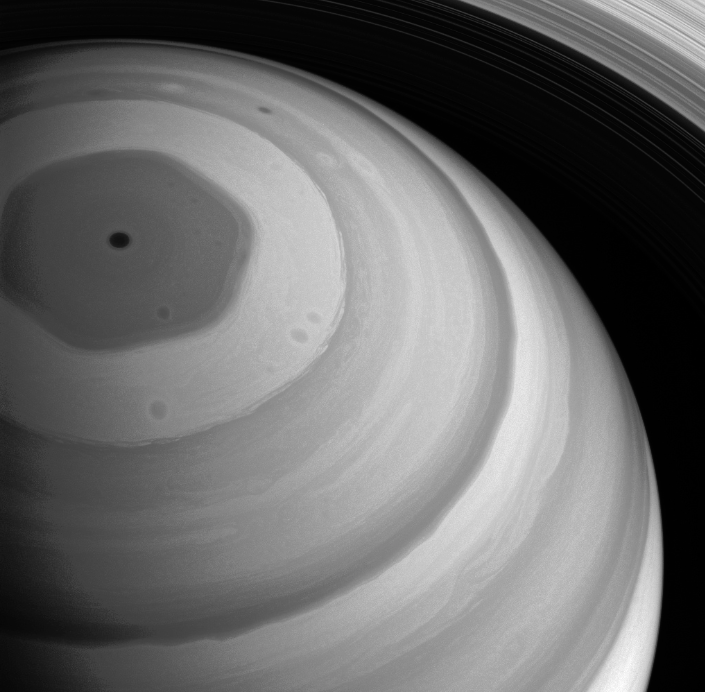
\includegraphics[width=3cm]{saturn-cassini_1.png}
\caption{カッシーニにより初めて観測された,六角形の北極域の模様.}
\end{figure}

\begin{figure}[htbp]
\centering
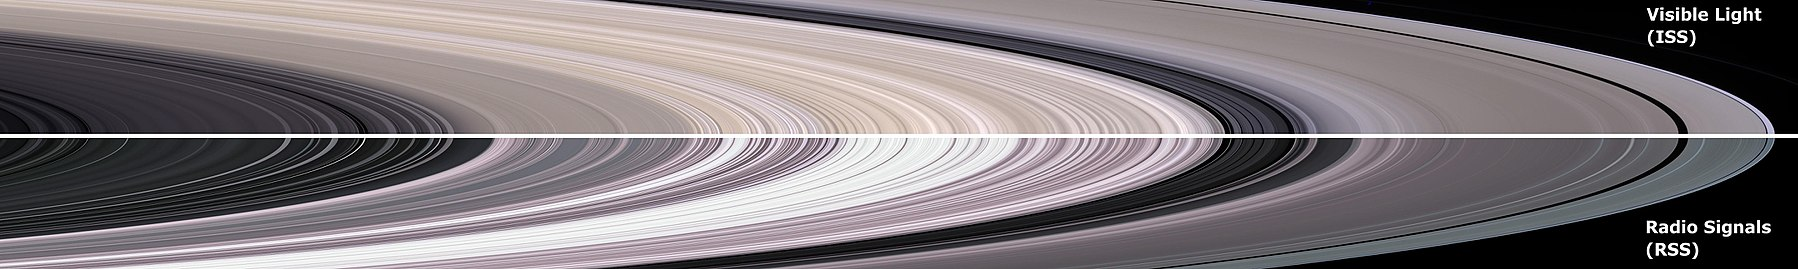
\includegraphics[width=10cm]{img/saturn-ring-cassini-2005.png}
\caption{カッシーニによる4度斜めから見たC環、B環及びA環の画像。上図は、2004年12月12日に撮影された無着色の画像.下図は2005年5月3日に撮影され、粒子の径に応じて彩色した画像.}
\end{figure}

\section{グランドフィナーレ}
グランドフィナーレというのは,2014年に発表された,カッシーニの最後のミッションである.
具体的には,土星とその環の「すきま」を22回にわたり周回し,近傍から土星の大気を調査,最後の周回を終えた後は,大気のサンプリングと地球へのデータ送信をしつつ,土星大気に突入し,「最期」を迎える,というものだ.
22回目の最後の周回は9月9日,文化祭1日目であり,「最期」は15日を予定している.
そのため,文化祭期間中には,展示の中で最新のカッシーニの情報も伝えていこうと思う.
\begin{figure}
\centering
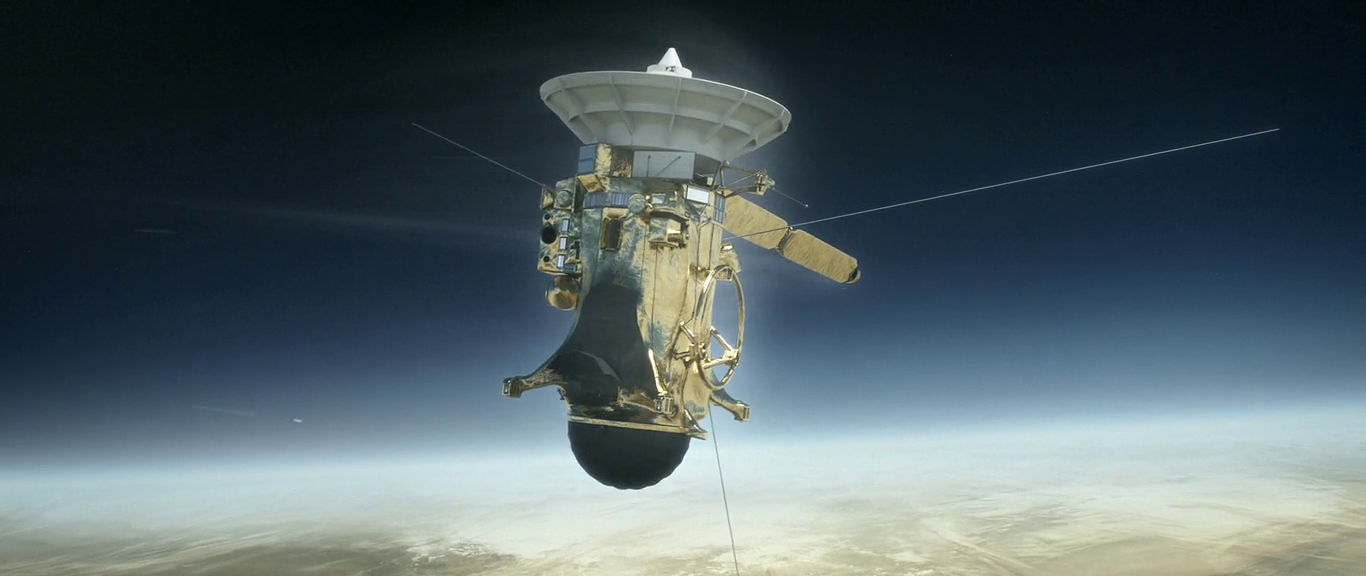
\includegraphics[width=10cm]{cassini-burn.jpg}
\caption{カッシーニはその役目を終えると,土星大気に突入して、燃え尽きる.}
\end{figure}


%\section{参考文献}
%https://ja.wikipedia.org/wiki/%E3%82%AB%E3%83%83%E3%82%B7%E3%83%BC%E3%83%8B_(%E6%8E%A2%E6%9F%BB%E6%A9%9F)
%https://www.nasa.gov/jpl/cassini/nasa-and-esa-celebrate-10-years-since-titan-landing
%https://www.nasa.gov/feature/jpl/new-movie-shows-cassinis-first-dive-over-saturn
%http://www.astronomy2009.jp/ja/webproject/life-g/08.html
%http://www.geocities.jp/planetnekonta2/hanasi/saturn/saturn.html
%https://www.astroarts.co.jp/special/2017saturn/index-j.shtml
%http://www.bbc.com/japanese/40920970
%http://solarviews.com/eng/saturnbg.htm
